\chapter{極低温環境用SOI-FETの \newline SPICE回路シミュレーター構築}
	SPICE(Simulation Program with Integrated Circuit Emphasis)とは電子回路をシミュレーションするソフトウェアであり、1972年アメリカのカリフォルニア大学バークレイ校で開発された。
	以後、回路図エディタ、波形表示機能など様々な改良や機能拡張を加えたSPICEは回路シミュレータ業界では業界標準となっており、回路設計のために全世界で使われている。
	
	回路シミュレーションのメリットとしては、
	\begin{itemize}
		\item シミュレーションの際に測定系をわざわざ構築せずに済むのでコストを抑えられる
		\item 上記から、同時に時間短縮もでき、素子破壊の危険などを回避することもできる
		\item 実測不可の測定系でも、シミュレーター上の理想的な測定環境を考察することが可能
	\end{itemize}
	などが挙げられる。
	
	我々研究グループはSTJ検出器信号を増幅するための極低温環境用SOI前置増幅器の研究開発を行っており、回路設計の際には入念な回路シミュレーションが必要不可欠である。
	しかし、現在極低温環境用SPICE回路シミュレータは存在していないのが現状である。
	そのため、我々は極低温環境下でのSPICE回路シミュレーター構築を行った。
	
	シミュレーター構築の流れは、
	\begin{enumerate}
		\item 常温環境下で様々なサイズのFD-SOI-MOSFETについての電流電圧特性を測定
		\item 極低温環境下において、常温環境下と同様に電流電圧特性を測定
		\item 得られた電流電圧特性から、モデリングに必要なパラメーターを抽出
	\end{enumerate}
	である。我々筑波大はKEK\ 倉地氏のご助力を頂きながら電流電圧特性の測定の方を行い、JAXA\ 馬場氏にパラメーター抽出をしていただいた。
	我々が設計する増幅器はNb/Al-STJ検出器が動作する環境での動作を想定しており、よって300mK環境用のSPICE回路シミュレーターを構築する必要がある。
	我々の今までの測定において、3K環境下、300mK環境下でのFD-SOI-MOSFETの電流電圧特性に違いはほぼないことがわかっている。
	したがって、本構築では便宜上3K環境用SPICE回路シミュレーターを構築することとする。
	
	以後、我々が測定したサンプルの性能評価についての結果、並びに馬場氏に抽出していただいたパラメータを元に構築された極低温環境用SPICEパラメーターと実測の比較について述べる。
	\clearpage
	\section{測定サンプル}
		我々が測定したサンプルは、MOSFETの構造の違いからBody-Tie(BT)型とSource-Tie2(ST2)型の2種類に大別できる。
		このBT型とST2型についての構造上の違いについて以下述べる。
		\begin{description}
			\item[Body-Tie型]\mbox{}\\
				Body部の接続端子が外部まで配線されているMOSFETのこと。
			\item[Source-Tie2型]\mbox{}\\
				Source-Tie型とは、Body部がSourceと電気的に接続されている構造を持つ。
				BodyとSourceが電気的に接続されているため浮遊容量を抑えることができる。\\
				このSource-Tie型にはSource-Tie(ST)型とSource-Tie2(ST2)型に大別でき、これはBodyとSourceが電気的に接続される場所と面積が異なる。
		\end{description}
		各MOSFETのIDとサイズについての詳細を表\ref{tab:BT_detail}と表\ref{tab:ST_detail}に示す。
		\begin{table}[htb]
			\begin{center}
				\begin{tabular}{| c | l | c | c |} \hline
					Device ID & Device Type & Channel Length & Channel Width \\ \hline \hline
					B1 & core nvt NMOS bt & $0.2 \mathrm{\mu m}$ & $0.4 \mathrm{\mu m}$ \\ \hline
					B2 & core nvt NMOS bt & $0.2 \mathrm{\mu m}$ & $5 \mathrm{\mu m}$ \\ \hline
					B3 & core nvt NMOS bt & $10 \mathrm{\mu m}$ & $5 \mathrm{\mu m}$ \\ \hline
					B4 & core nvt NMOS bt & $10 \mathrm{\mu m}$ & $0.4 \mathrm{\mu m}$ \\ \hline \hline
					B5 & core nvt PMOS bt & $0.2 \mathrm{\mu m}$ & $0.5 \mathrm{\mu m}$ \\ \hline
					B6 & core nvt PMOS bt & $0.2 \mathrm{\mu m}$ & $5 \mathrm{\mu m}$ \\ \hline
					B7 & core nvt PMOS bt & $10 \mathrm{\mu m}$ & $5 \mathrm{\mu m}$ \\ \hline
					B8 & core nvt PMOS bt & $10 \mathrm{\mu m}$ & $0.63 \mathrm{\mu m}$ \\ \hline
				\end{tabular}
				\caption{測定したBody-Tie型FD-SOI-MOSFETの詳細}
				\label{tab:BT_detail}
			\end{center}
		\end{table}
		
		\begin{table}[htb]
			\begin{center}
				\begin{tabular}{| c | l | c | c |} \hline
					Device ID & Device Type & Channel Length & Channel Width \\ \hline \hline
					NS1 & core lvt NMOS st2 & $0.4 \mathrm{\mu m}$ & $1 \mathrm{\mu m}$ \\ \hline
					NS2 & core lvt NMOS st2 & $0.4 \mathrm{\mu m}$ & $2 \mathrm{\mu m}$ \\ \hline
					NS3 & core lvt NMOS st2 & $0.4 \mathrm{\mu m}$ & $10 \mathrm{\mu m}$ \\ \hline
					NS4 & core lvt NMOS st2 & $1 \mathrm{\mu m}$ & $10 \mathrm{\mu m}$ \\ \hline
					NS5 & core lvt NMOS st2 & $5 \mathrm{\mu m}$ & $10 \mathrm{\mu m}$ \\ \hline
					NS6 & core lvt NMOS st2 & $1 \mathrm{\mu m}$ & $1 \mathrm{\mu m}$ \\ \hline
					NS7 & core lvt NMOS st2 & $5 \mathrm{\mu m}$ & $1 \mathrm{\mu m}$ \\ \hline
					NS8 & core lvt NMOS st2 & $1 \mathrm{\mu m}$ & $2 \mathrm{\mu m}$ \\ \hline \hline
					PS1 & core lvt PMOS st2 & $0.4 \mathrm{\mu m}$ & $1 \mathrm{\mu m}$ \\ \hline
					PS2 & core lvt PMOS st2 & $0.4 \mathrm{\mu m}$ & $2 \mathrm{\mu m}$ \\ \hline
					PS3 & core lvt PMOS st2 & $0.4 \mathrm{\mu m}$ & $10 \mathrm{\mu m}$ \\ \hline
					PS4 & core lvt PMOS st2 & $1 \mathrm{\mu m}$ & $10 \mathrm{\mu m}$ \\ \hline
					PS5 & core lvt PMOS st2 & $5 \mathrm{\mu m}$ & $10 \mathrm{\mu m}$ \\ \hline
					PS6 & core lvt PMOS st2 & $1 \mathrm{\mu m}$ & $1 \mathrm{\mu m}$ \\ \hline
					PS7 & core lvt PMOS st2 & $5 \mathrm{\mu m}$ & $1 \mathrm{\mu m}$ \\ \hline
					PS8 & core lvt PMOS st2 & $1 \mathrm{\mu m}$ & $2 \mathrm{\mu m}$ \\ \hline
				\end{tabular}
				\caption{測定したSource-Tie型FD-SOI-MOSFETの詳細}
				\label{tab:ST_detail}
			\end{center}
		\end{table}
		\clearpage

	\section{電流電圧特性\ 測定環境}
		\subsection{測定系}
			\begin{figure}[htbp]
				\begin{center}
					\includegraphics[width=12.0cm]{./Chapter/Chapter5/Picture/IVmeasurement_circuit.eps}
					\caption{MOSFETの電流電圧特性の測定回路図(NMOSFETの場合)}
					\label{fig:IVmeasurement_circuit}
				\end{center}
			\end{figure}
			\begin{table}[htb]
				\begin{center}
					\begin{tabular}{| c | c | c |} \hline
						材質 & 配線抵抗$R_{refregerator}$ & 配線容量$C_{refregerator}$ \\ \hline \hline
						コンスタンタン & 約$70 \mathrm{\Omega}$程度 & 約$0.5 \mathrm{nF}$程度 \\ \hline
					\end{tabular}
					\caption{$\mathrm{^{3}He}$減圧冷凍機 読み出し配線の詳細}
					\label{tab:refregerator_wire}
				\end{center}
			\end{table}
			MOSFETの電流電圧特性の測定回路図を図\ref{fig:IVmeasurement_circuit}に示す。
			MOSFETを冷凍機内に設置し、長い冷凍機配線を経て室温に読み出し線を出す。この読み出し配線の詳細についてを表\ref{tab:refregerator_wire}にまとめた。\\
			電流電圧特性の測定にはソースメータ(KEITHLEY 2401)を用いた。
			PC上で各端子に印加する電圧を設定し、GPIBを介して各ソースメーターがMOSFETの各端子に電圧を印加し、そのときの電流値を測定するように命令を送る。
			そのときの測定値をPC上に保存するようにした。
		\subsection{測定項目}
			各デバイスごとに測定した電流電圧特性は、
			\begin{itemize}
				\item ドレイン電流のゲート電圧依存性($I_{ds}-V_{gs}$特性)
				\item ドレイン電流のドレイン電圧依存性($I_{ds}-V_{ds}$特性)
			\end{itemize}
			の2種類である。それぞれの依存性について常温環境下、3K環境下それぞれ測定した。\\
			以下2つのドレイン電流のバイアス電圧依存性の測定の際に印加した電圧について、MOSFETのタイプごとに表に示した。
			\begin{table}[htb]
				\begin{center}
					\begin{tabular}{| l c |} \hline \hline
						{\bf $I_{ds}-V_{gs}$特性} & \ \\ \hline
						$V_{body}\ =\  0\ \mathrm{V}$ & \ \\
						$V_{source}\ =\ 0\ \mathrm{V}$ & \ \\
						$V_{d}\ =\ 0.05\ /\ 1.8\ \mathrm{V}$ & 2\ points \\
						$V_{g}\ =\ 0\ \mathrm{V}\ \mathrm{to}\ 2\ \mathrm{V}$\ \ Step\ $0.02\ \mathrm{V}$ & 101\ points \\ \hline \hline
						{\bf $I_{ds}-V_{ds}$特性} & \ \\ \hline
						$V_{body}\ =\  0\ \mathrm{V}$ & \ \\
						$V_{source}\ =\ 0\ \mathrm{V}$ & \ \\
						$V_{g}\ =\ 0\ /\ 0.4\ /\ 0.8\ /\ 1.2\ /\ 1.6\ /\ 2.0\ \mathrm{V}$ & 6\ points \\
						$V_{d}\ =\ 0\ \mathrm{V}\ \mathrm{to}\ 2\ \mathrm{V}$\ \ Step\ $0.1\ \mathrm{V}$ & 21\ points \\ \hline
					\end{tabular}
					\caption{MOSFET(Device Type : core nvt NMOS Body-Tie)の電流電圧特性測定\\各電圧のパラメータ}
					\label{tab:NBT_bias}
				\end{center}
			\end{table}

			\begin{table}[htb]
				\begin{center}
					\begin{tabular}{| l c |} \hline \hline
						{\bf $I_{ds}-V_{gs}$特性} & \ \\ \hline
						$V_{body}\ =\  1.8\ \mathrm{V}$ & \ \\
						$V_{source}\ =\ 1.8\ \mathrm{V}$ & \ \\
						$V_{d}\ =\ 1.75\ /\ 0\ \mathrm{V}$ & 2\ points \\
						$V_{g}\ =\ 1.8\ \mathrm{V}\ \mathrm{to}\ -0.2\ \mathrm{V}$\ \ Step\ $-0.02\ \mathrm{V}$ & 101\ points \\ \hline \hline
						{\bf $I_{ds}-V_{ds}$特性} & \ \\ \hline
						$V_{body}\ =\  1.8\ \mathrm{V}$ & \ \\
						$V_{source}\ =\ 1.8\ \mathrm{V}$ & \ \\
						$V_{g}\ =\ 1.8\ /\ 1.4\ /\ 1.0\ /\ 0.6\ /\ 0.2\ /\ -0.2\ \mathrm{V}$ & 6\ points \\
						$V_{d}\ =\ 1.8\ \mathrm{V}\ \mathrm{to}\ -0.2\ \mathrm{V}$\ \ Step\ $-0.1\ \mathrm{V}$ & 21\ points \\ \hline
					\end{tabular}
					\caption{MOSFET(Device Type : core nvt PMOS Body-Tie)の電流電圧特性測定\\各電圧のパラメータ}
					\label{tab:PBT_bias}
				\end{center}
			\end{table}
			
			\begin{table}[htb]
				\begin{center}
					\begin{tabular}{| l c |} \hline \hline
						{\bf $I_{ds}-V_{gs}$特性} & \ \\ \hline
						$V_{source}\ =\ 0\ \mathrm{V}$ & \ \\
						$V_{d}\ =\ 0.05\ /\ 1.8\ \mathrm{V}$ & 2\ points \\
						$V_{g}\ =\ 0\ \mathrm{V}\ \mathrm{to}\ 2\ \mathrm{V}$\ \ Step\ $0.02\ \mathrm{V}$ & 101\ points \\ \hline \hline
						{\bf $I_{ds}-V_{ds}$特性} & \ \\ \hline
						$V_{source}\ =\ 0\ \mathrm{V}$ & \ \\
						$V_{g}\ =\ 0\ /\ 0.4\ /\ 0.8\ /\ 1.2\ /\ 1.6\ /\ 2.0\ \mathrm{V}$ & 6\ points \\
						$V_{d}\ =\ 0\ \mathrm{V}\ \mathrm{to}\ 2\ \mathrm{V}$\ \ Step\ $0.1\ \mathrm{V}$ & 21\ points \\ \hline
					\end{tabular}
					\caption{MOSFET(Device Type : core lvt NMOS Source-Tie)の電流電圧特性測定\\各電圧のパラメータ}
					\label{tab:NST_bias}
				\end{center}
			\end{table}

			\begin{table}[htb]
				\begin{center}
					\begin{tabular}{| l c |} \hline \hline
						{\bf $I_{ds}-V_{gs}$特性} & \ \\ \hline
						$V_{source}\ =\ 1.8\ \mathrm{V}$ & \ \\
						$V_{d}\ =\ 1.75\ /\ 0\ \mathrm{V}$ & 2\ points \\
						$V_{g}\ =\ 1.8\ \mathrm{V}\ \mathrm{to}\ -0.2\ \mathrm{V}$\ \ Step\ $-0.02\ \mathrm{V}$ & 101\ points \\ \hline \hline
						{\bf $I_{ds}-V_{ds}$特性} & \ \\ \hline
						$V_{source}\ =\ 1.8\ \mathrm{V}$ & \ \\
						$V_{g}\ =\ 1.8\ /\ 1.4\ /\ 1.0\ /\ 0.6\ /\ 0.2\ /\ -0.2\ \mathrm{V}$ & 6\ points \\
						$V_{d}\ =\ 1.8\ \mathrm{V}\ \mathrm{to}\ -0.2\ \mathrm{V}$\ \ Step\ $-0.1\ \mathrm{V}$ & 21\ points \\ \hline
					\end{tabular}
					\caption{MOSFET(Device Type : core lvt PMOS Source-Tie)の電流電圧特性測定\\各電圧のパラメータ}
					\label{tab:PST_bias}
				\end{center}
			\end{table}
			\clearpage 

	\section{電流電圧特性\ 測定結果}
		まず常温環境下でMOSFETの電流電圧特性の測定を行った。
		MOSFETの各端子に印加する電圧のパラメータはDevice Typeごとに表\ref{tab:NBT_bias}〜表\ref{tab:PST_bias}に記した。
		本節では、FD-SOI-MOSFETの型ごとに測定結果を述べる。
		\subsection{Body Tie型}
			Body Tie型のMOSFETの電流電圧特性を図\ref{fig:BT_N_IdVg}と図\ref{fig:BT_N_IdVd}に示す。
			
			図\ref{fig:BT_N_IdVg}は$I_{ds}-V_{gs}$特性を示す。図\ref{fig:BT_N_IdVg}[a]は常温環境下、図\ref{fig:BT_N_IdVg}[b]は3K環境下での特性を示す。
			両者を比較すると、
			\begin{itemize}
				\item 低温になるほど閾電圧の上昇
				\item サブスレッショルド領域でのドレイン電流の急激な上昇
			\end{itemize}
			を確認できた。
			
			また、図\ref{fig:BT_N_IdVd}は$I_{ds}-V_{ds}$特性を示す。図\ref{fig:BT_N_IdVd}[a]は常温環境下、図\ref{fig:BT_N_IdVd}[b]は3K環境下での特性を示す。
			先程と同様に両者を比較すると、
			\begin{itemize}
				\item 低温になるほど、飽和電流値の上昇
				\item 3K環境下において、ドレイン電圧が低い領域においてドレイン電流の立ち上がりの鈍化
				\item 3K環境下において、ドレイン電圧が高い領域においてドレイン電流の急な上昇
			\end{itemize}
			を確認できた。

			%=====Ids-Vgs特性=====%
			\begin{figure}[htbp]
				\begin{center}
					\begin{tabular}{c}
						%1
						\begin{minipage}{0.5\hsize}
							\begin{center}
								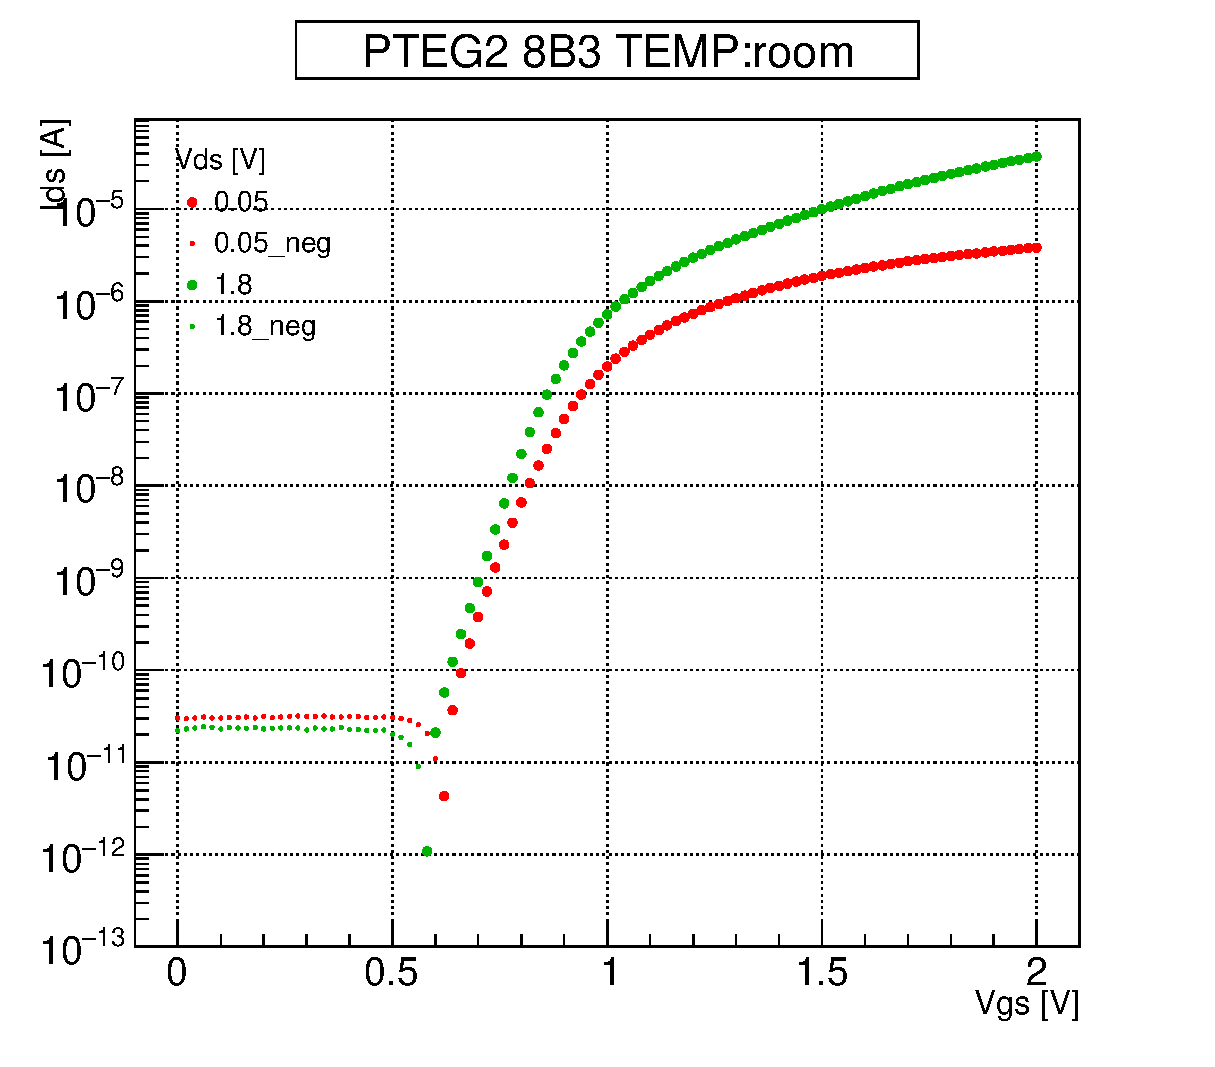
\includegraphics[clip, width=6cm]{./Chapter/Appendix/Picture/NBT/B3/PTEG2_8_B3_IdVg_room.eps}
								\hspace{1.6cm} [a]常温環境下
							\end{center}
						\end{minipage}
						%2
						\begin{minipage}{0.5\hsize}
							\begin{center}
								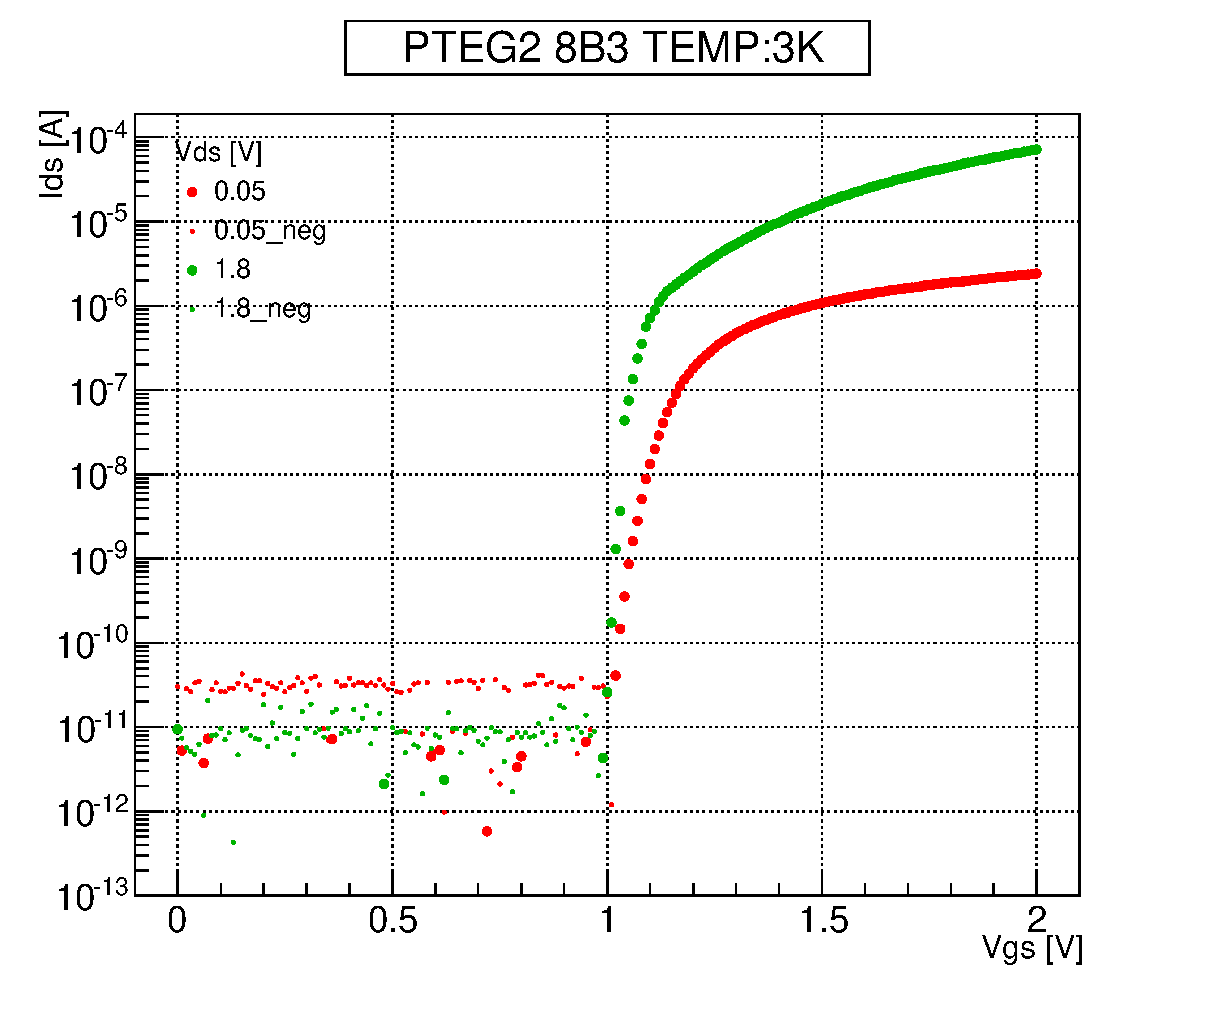
\includegraphics[clip, width=6cm]{./Chapter/Appendix/Picture/NBT/B3/PTEG2_8_B3_IdVg_3K.eps}
								\hspace{1.6cm} [b]3K環境下
							\end{center}
						\end{minipage}
					\end{tabular}
					\caption{Body Tie型(NMOS)の$I_{ds}-V_{gs}$特性\ Device ID : B3($W/L = 0.4\mathrm{\mu m} / 0.2\mathrm{\mu m}$)}
					\label{fig:BT_N_IdVg}
				\end{center}
			\end{figure}
			%=====Ids-Vds特性=====%
			\begin{figure}[htbp]
				\begin{center}
					\begin{tabular}{c}
						%1
						\begin{minipage}{0.5\hsize}
							\begin{center}
								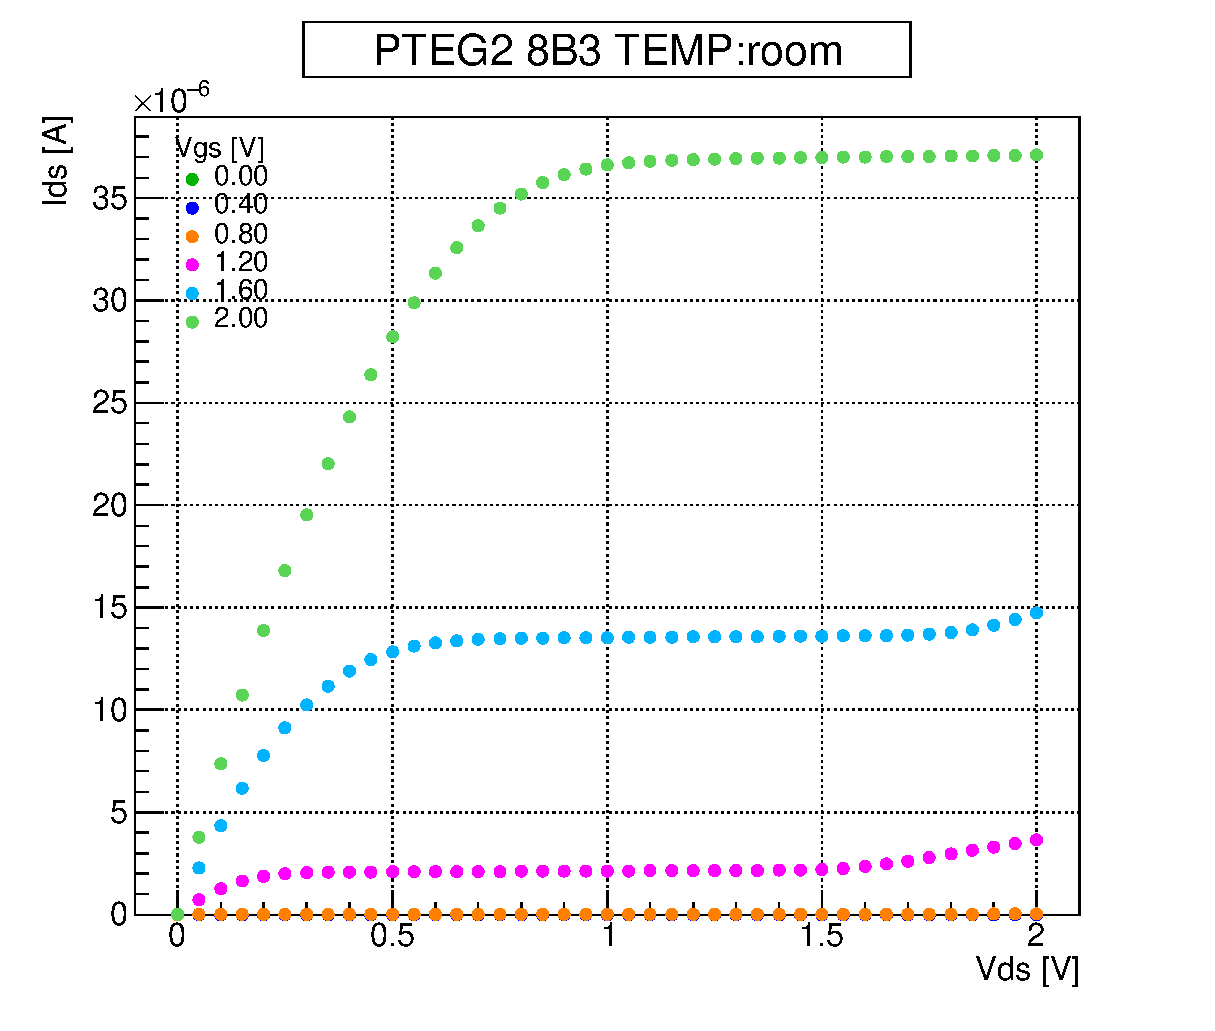
\includegraphics[clip, width=6cm]{./Chapter/Appendix/Picture/NBT/B3/PTEG2_8_B3_IdVd_room.eps}
								\hspace{1.6cm} [a]常温環境下
							\end{center}
						\end{minipage}
						%2
						\begin{minipage}{0.5\hsize}
							\begin{center}
								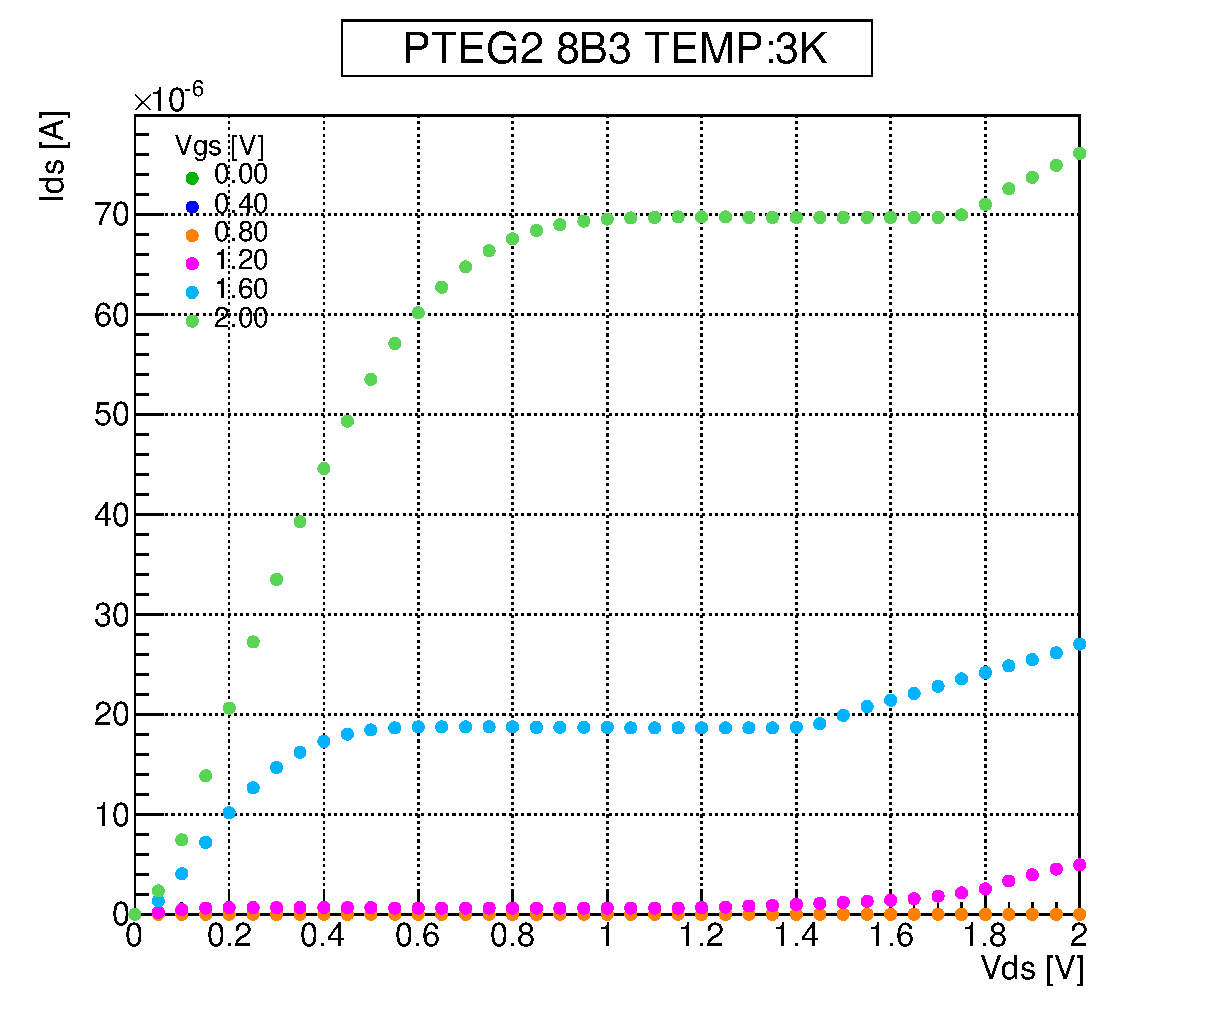
\includegraphics[clip, width=6cm]{./Chapter/Appendix/Picture/NBT/B3/PTEG2_8_B3_IdVd_3K.eps}
								\hspace{1.6cm} [b]3K環境下
							\end{center}
						\end{minipage}
					\end{tabular}
					\caption{Body Tie型(NMOS)の$I_{ds}-V_{ds}$特性\ Device ID : B3($W/L = 0.4\mathrm{\mu m} / 0.2\mathrm{\mu m}$)}
					\label{fig:BT_N_IdVd}
				\end{center}
			\end{figure}
			
			\clearpage
			
		\subsection{Source-Tie2型}
		ST2型の電流電圧測定結果を図\ref{fig:ST_N_IdVg}と図\ref{fig:ST_N_IdVd}に示す。
		BT型と構造の異なるMOSFETでも、同様の電流電圧特性が現れていることを確認できた。
		
		また、全サンプルに対して、BT型と同様の電流電圧特性が現れていることを確認した。
		各Device Typeごとの全電流電圧特性の測定結果については、付録A章に示した。
		
		以上の結果をもとに我々は極低温環境下でのMOSFETの振る舞いについて調べた。
		我々が極低温環境下で用いるFD-SOI-MOSFETはST2型なので、以降の解析ではST2型についての解析のみ触れることにする。
			%=====Ids-Vgs特性=====%
			\begin{figure}[htbp]
				\begin{center}
					\begin{tabular}{c}
						%1
						\begin{minipage}{0.5\hsize}
							\begin{center}
								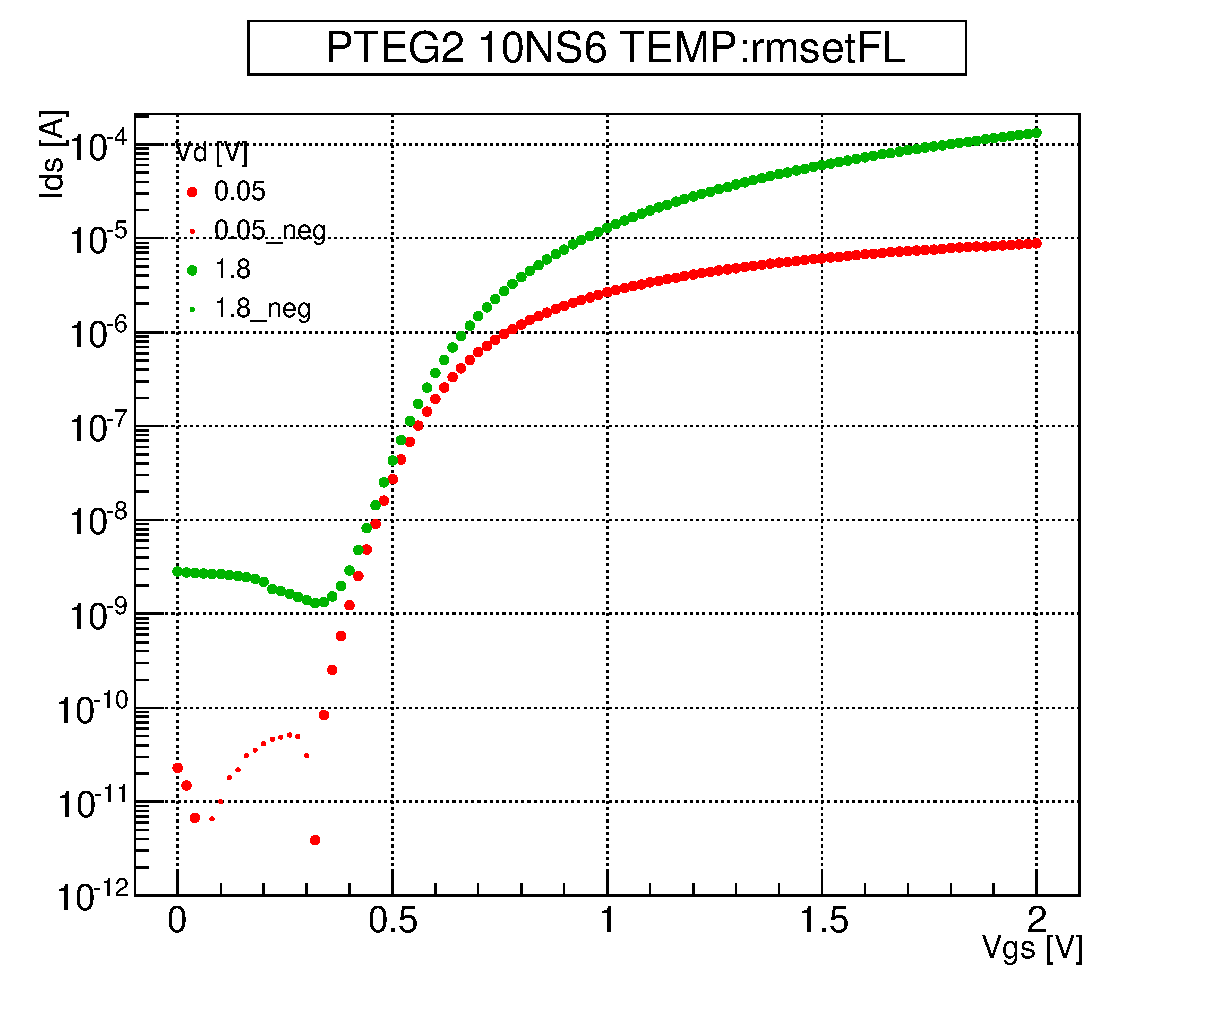
\includegraphics[clip, width=6cm]{./Chapter/Appendix/Picture/NST/NS6/PTEG2_10_NS6_IdVg_rmsetFL.eps}
								\hspace{1.6cm} [a]常温環境下
							\end{center}
						\end{minipage}
						%2
						\begin{minipage}{0.5\hsize}
							\begin{center}
								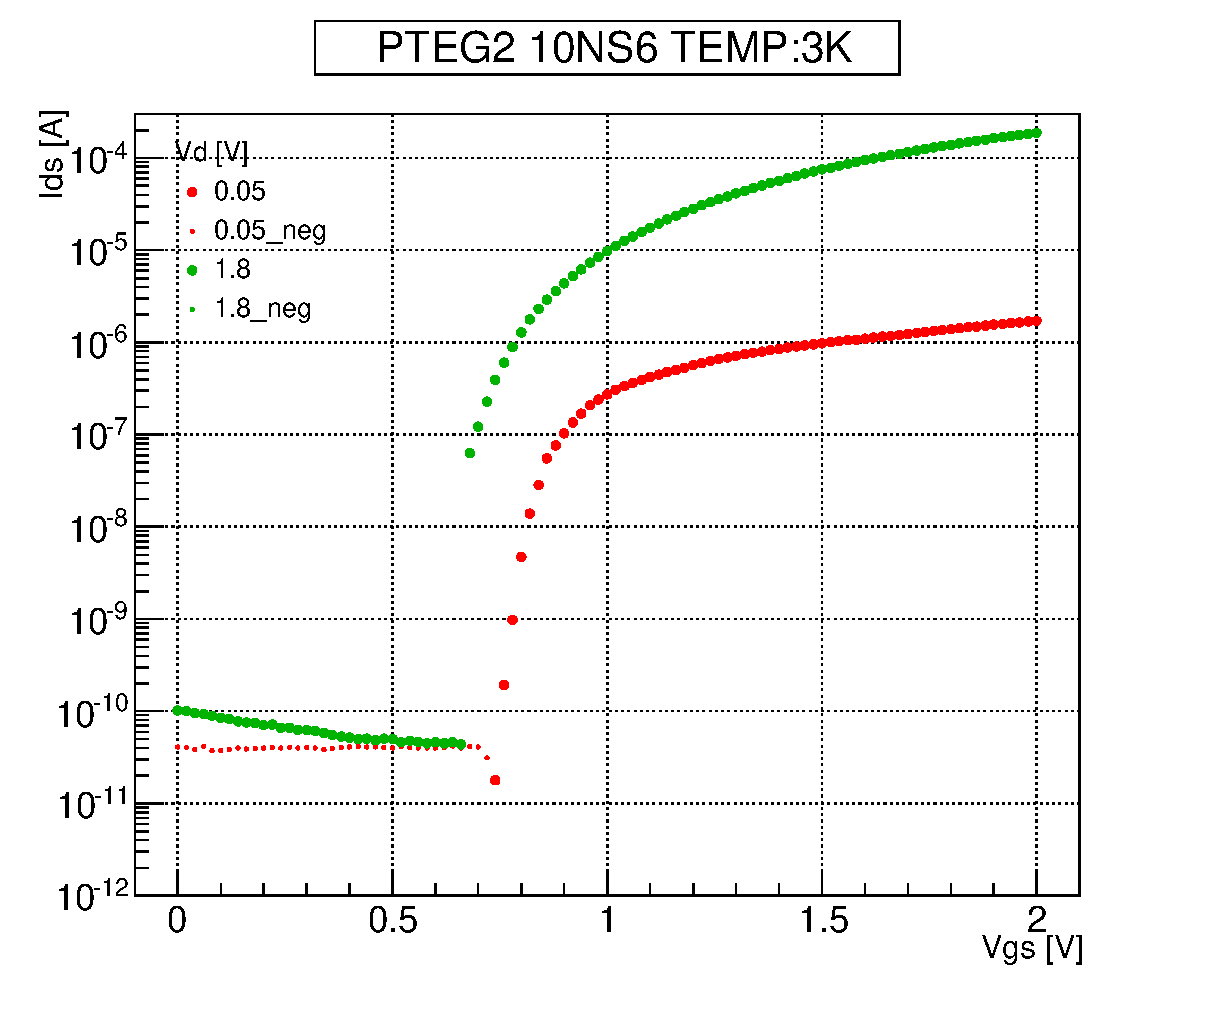
\includegraphics[clip, width=6cm]{./Chapter/Appendix/Picture/NST/NS6/PTEG2_10_NS6_IdVg_3K.eps}
								\hspace{1.6cm} [b]3K環境下
							\end{center}
						\end{minipage}
					\end{tabular}
					\caption{Source Tie型(NMOS)の$I_{ds}-V_{gs}$特性\ Device ID : NS6($W/L = 1\mathrm{\mu m} / 1\mathrm{\mu m}$)}
					\label{fig:ST_N_IdVg}
				\end{center}
			\end{figure}
			%=====Ids-Vds特性=====%
			\begin{figure}[htbp]
				\begin{center}
					\begin{tabular}{c}
						%1
						\begin{minipage}{0.5\hsize}
							\begin{center}
								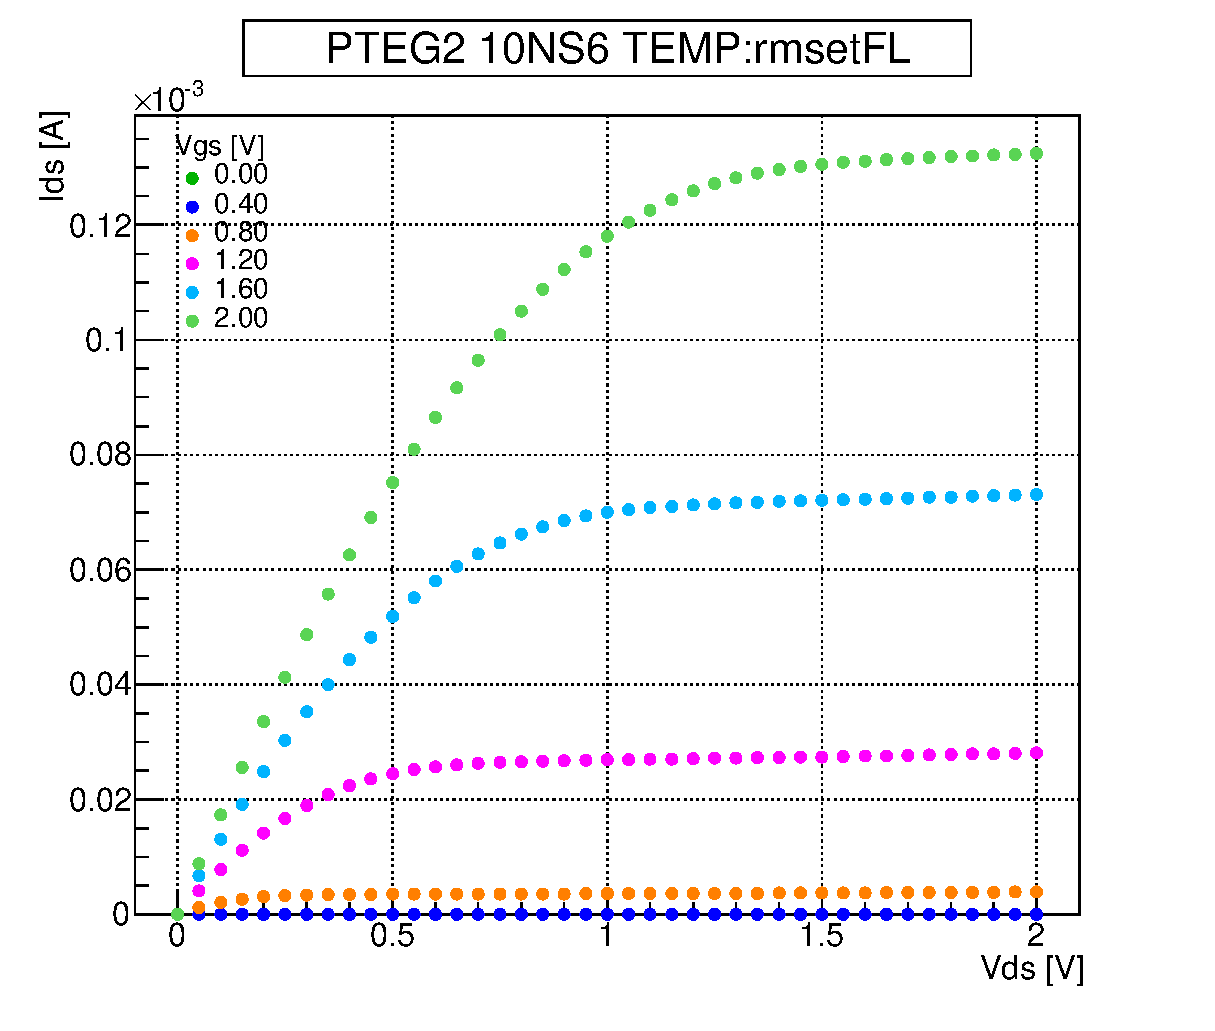
\includegraphics[clip, width=6cm]{./Chapter/Appendix/Picture/NST/NS6/PTEG2_10_NS6_IdVd_rmsetFL.eps}
								\hspace{1.6cm} [a]常温環境下
							\end{center}
						\end{minipage}
						%2
						\begin{minipage}{0.5\hsize}
							\begin{center}
								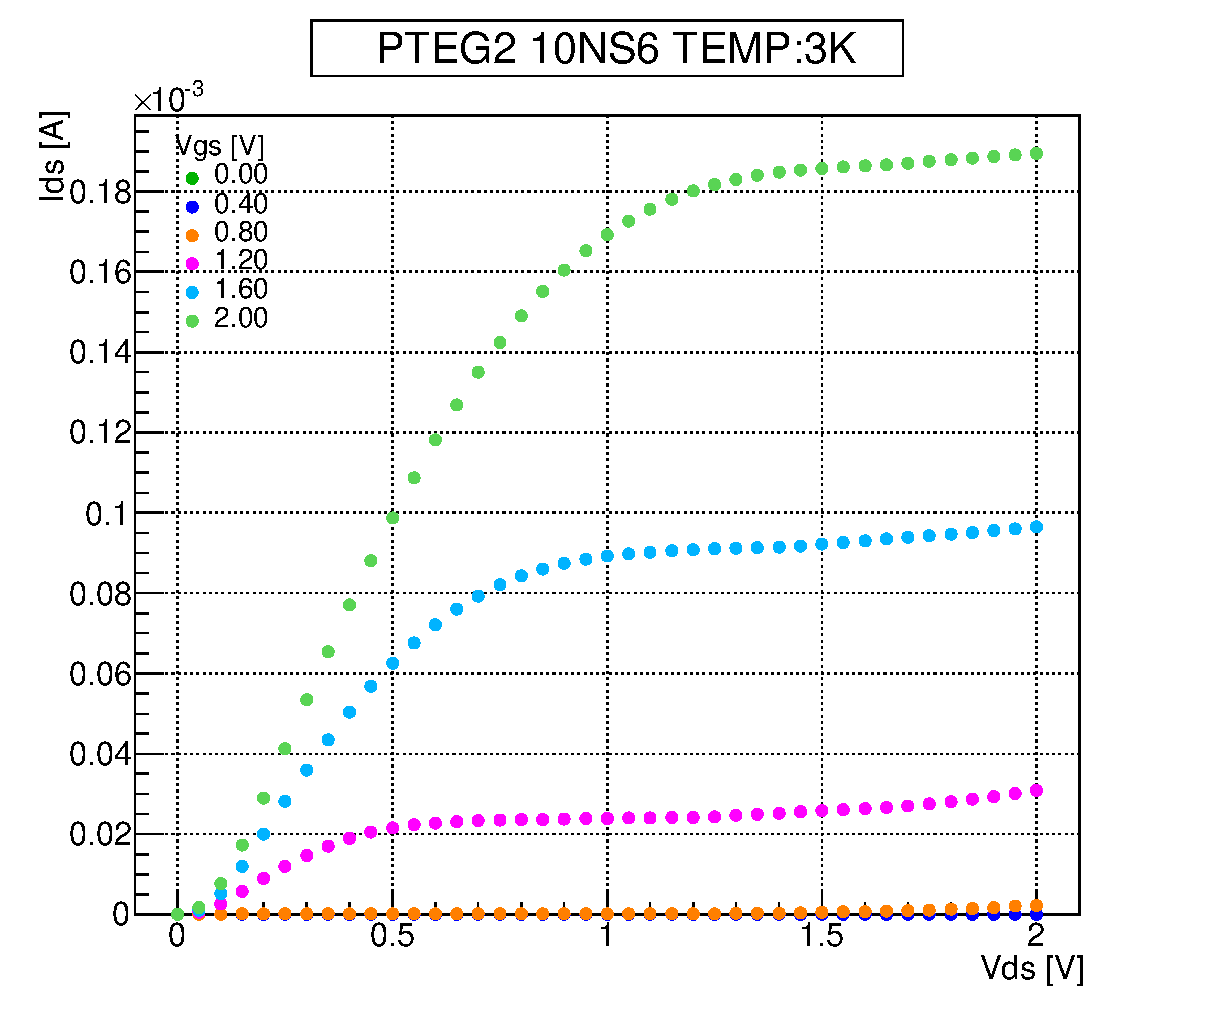
\includegraphics[clip, width=6cm]{./Chapter/Appendix/Picture/NST/NS6/PTEG2_10_NS6_IdVd_3K.eps}
								\hspace{1.6cm} [b]3K環境下
							\end{center}
						\end{minipage}
					\end{tabular}
					\caption{Source Tie型(NMOS)の$I_{ds}-V_{ds}$特性\ Device ID : NS6($W/L = 1\mathrm{\mu m} / 1\mathrm{\mu m}$)}
					\label{fig:ST_N_IdVd}
				\end{center}
			\end{figure}

		
	\section{解析}
		\subsection{閾値電圧の温度依存性}
			ゲート界面の電位が高くなると、ゲート直下のボディ部の半導体の型が反転する。
			それに伴いドレイン電流が流れ始め、トランジスタとしては「オン」の状態になる。
			
			しかし、実際にはゲート電圧が高くなるに従ってMOSFETは徐々にオンの状態になるので、閾値電圧を明確に定義するのは非常に困難である。
			そこで我々はゲート電圧が閾値電圧になるときのドレイン電流を式(\ref{eq:Vth_definition})のように定義した。
			\begin{eqnarray}
				I_{ds} = 0.1[\mathrm{\mu A}] \times \frac{W}{L}
				\label{eq:Vth_definition}
			\end{eqnarray}
			
			この式(\ref{eq:Vth_definition})に従って、常温環境下と極低温環境下において閾値電圧の変動を検証した。
			検証した結果の各サンプルごとの閾値電圧を表\ref{tab:Vth_temp}にまとめた。
			どのサンプルも閾値電圧は室温時と比較して、3K時の閾値電圧の方が約0.2V程度高くなることがわかる。
			例として、図\ref{fig:ST_N_IdVg_Vth}に$I_{ds}-V_{gs}$特性を常温環境下と3K環境下で比較したサンプルを例として示す。
			%=====
			\begin{table}[htb]
			\centering
				\begin{tabular}{|c|cc|c|cc|cc|}
					\hline
					\multirow{3}{*}{ID} & \multirow{3}{*}{L[$\mathrm{\mu m}$]} & \multirow{3}{*}{W[$\mathrm{\mu m}$]} & \multirow{3}{*}{$I_{ds}(V_{gs}=V_{th})$A} & \multicolumn{2}{c|}{Room} & \multicolumn{2}{c|}{3K} \\ \cline{5-8} 
					 &  &  &  & \multicolumn{1}{c|}{$V_{ds} = 0.05V$} & $V_{ds} = 1.80V$ & \multicolumn{1}{c|}{$V_{ds} = 0.05$V} & $V_{ds} = 1.80$V \\
					 &  &  &  & \multicolumn{1}{c|}{$V_{th}$} & $V_{th}$ & \multicolumn{1}{c|}{$V_{th}$} & $V_{th}$ \\ \hline
					NS1 & 0.4 & 1 & $4 \times 10^{-8}$ & 0.64 & 0.59 & 0.97 & 0.77 \\
					NS2 & 0.4 & 2 & $2 \times 10^{-8}$ & 0.58 & 0.53 & 0.91 & 0.61 \\
					NS3 & 0.4 & 10 & $4 \times 10^{-9}$ & 0.59 & 0.55 & 0.95 & 0.63 \\
					NS4 & 1 & 10 & $1 \times 10^{-8}$ & 0.61 & 0.59 & 0.85 & 0.63 \\
					NS5 & 5 & 10 & $5 \times 10^{-8}$ & 0.61 & 0.61 & 0.81 & 0.69 \\
					NS6 & 1 & 1 & $1 \times 10^{-7}$ & 0.56 & 0.53 & 0.89 & 0.69 \\
					NS7 & 5 & 1 & $5 \times 10^{-7}$ & 0.60 & 0.57 & 0.93 & 0.79 \\
					NS8 & 1 & 2 & $5 \times 10^{-8}$ & 0.59 & 0.51 & 0.87 & 0.69 \\ \hline
				\end{tabular}
				\caption{各サイズごとの閾値電圧$V_{th}$の温度依存性(NMOS Source Tie2型)}
				\label{tab:Vth_temp}
			\end{table}
			\clearpage
			
			\begin{figure}[htbp]
				\begin{center}
					\begin{tabular}{c}
						%1
						\begin{minipage}{0.5\hsize}
							\begin{center}
								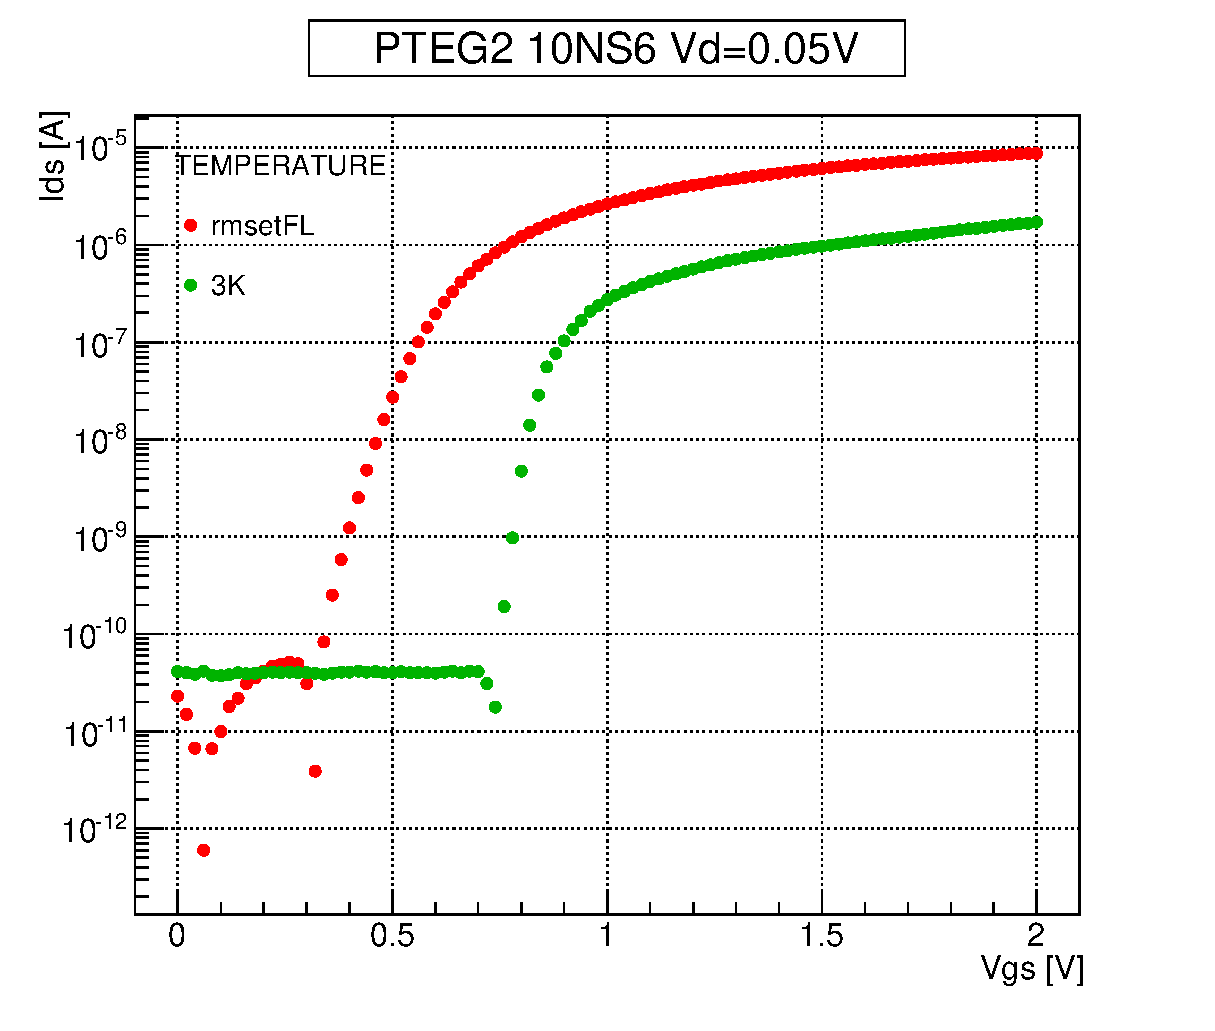
\includegraphics[clip, width=6.5cm]{./Chapter/Appendix/Picture/NST/NS6/PTEG10_NS6_IdVg_0.05_.log_.eps}
								\hspace{1.6cm} [a]ドレイン電圧$V_{ds}=0.05\mathrm{V}$
							\end{center}
						\end{minipage}
						%2
						\begin{minipage}{0.5\hsize}
							\begin{center}
								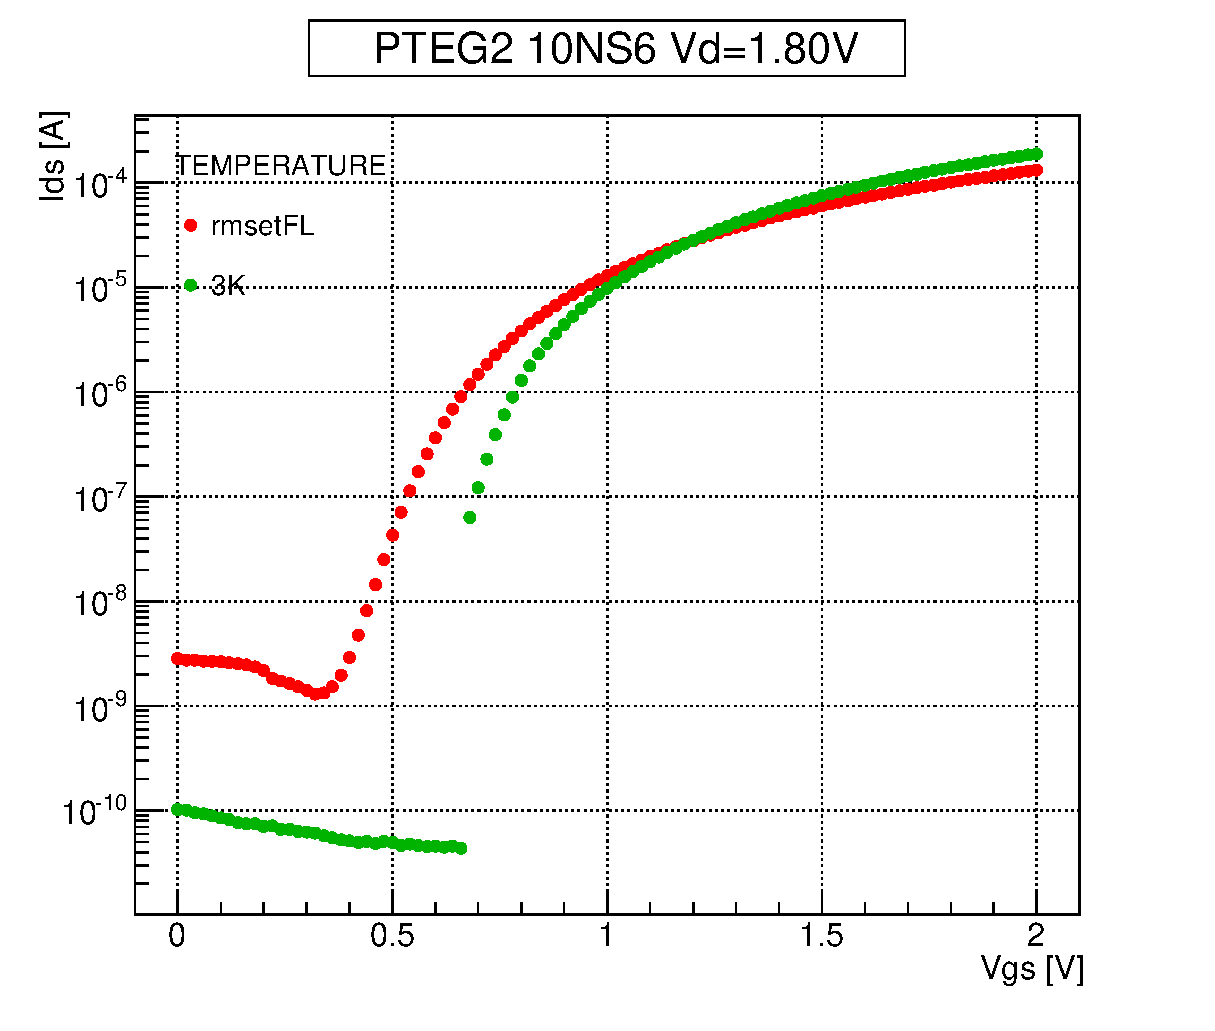
\includegraphics[clip, width=6.5cm]{./Chapter/Appendix/Picture/NST/NS6/PTEG10_NS6_IdVg_1.80_.log_.eps}
								\hspace{1.6cm} [b]ドレイン電圧$V_{ds}=1.80\mathrm{V}$
							\end{center}
						\end{minipage}
					\end{tabular}
					\caption{Source Tie型(NMOS)の$I_{ds}-V_{gs}$特性(縦軸 : 対数表示)\ Device ID : NS6($W/L = 1\mathrm{\mu m} / 1\mathrm{\mu m}$)}
					\label{fig:ST_N_IdVg_Vth}
				\end{center}
			\end{figure}
			
			\begin{figure}[htbp]
				\begin{center}
					\begin{tabular}{c}
						%1
						\begin{minipage}{0.5\hsize}
							\begin{center}
								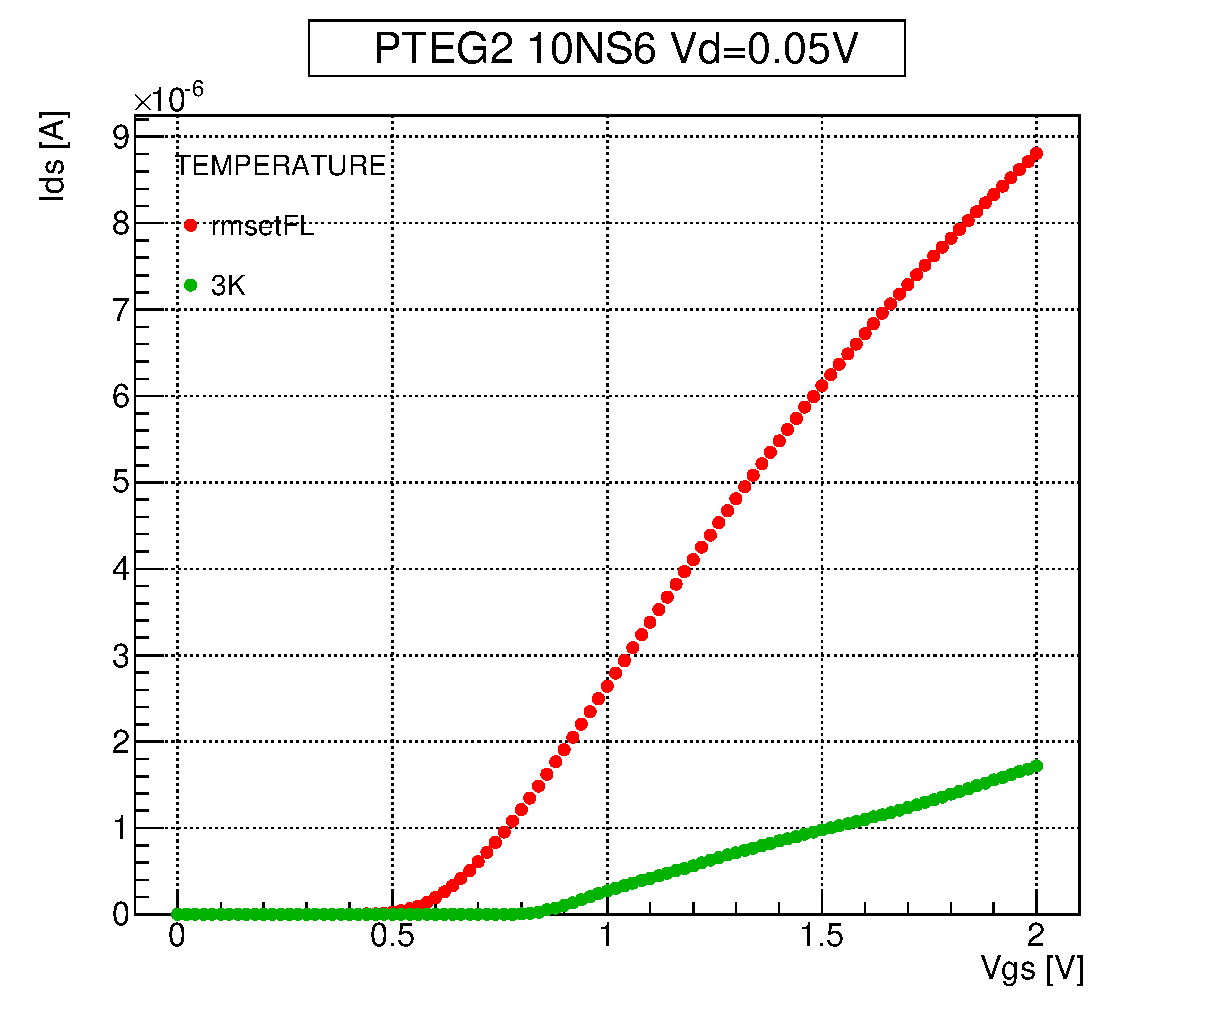
\includegraphics[clip, width=6.5cm]{./Chapter/Appendix/Picture/NST/NS6/PTEG10_NS6_IdVg_0.05_.linear_.eps}
								\hspace{1.6cm} [a]ドレイン電圧$V_{ds}=0.05\mathrm{V}$
							\end{center}
						\end{minipage}
						%2
						\begin{minipage}{0.5\hsize}
							\begin{center}
								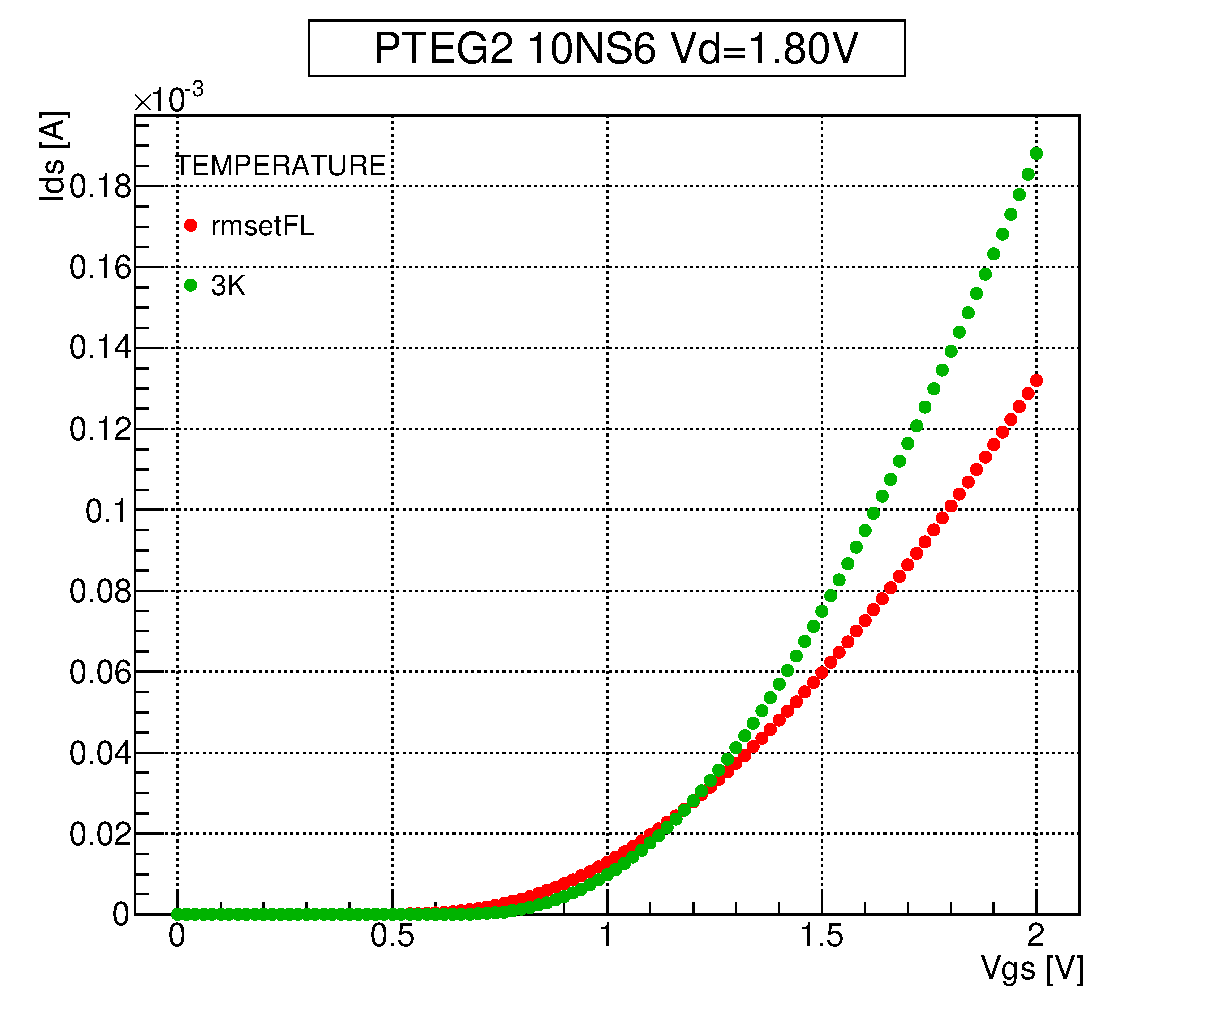
\includegraphics[clip, width=6.5cm]{./Chapter/Appendix/Picture/NST/NS6/PTEG10_NS6_IdVg_1.80_.linear_.eps}
								\hspace{1.6cm} [b]ドレイン電圧$V_{ds}=1.80\mathrm{V}$
							\end{center}
						\end{minipage}
					\end{tabular}
					\caption{Source Tie型(NMOS)の$I_{ds}-V_{gs}$特性(縦軸 : 線形表示)\ Device ID : NS6($W/L = 1\mathrm{\mu m} / 1\mathrm{\mu m}$)}
					\label{fig:ST_N_IdVg_Vth}
				\end{center}
			\end{figure}
			\clearpage

		\subsection{飽和電流値の温度依存性}
			飽和領域での飽和電流値はチャネル長変調効果を無視すると、式(\ref{eq:Ids_saturate})のように書くことができる。
			\begin{eqnarray}
				I_{ds} = \frac{1}{2} \mu(T) C_{OX} \frac{W}{L} {(V_{gs} - V_{th})}^2
				\label{eq:Ids_saturate}
			\end{eqnarray}
			ゲートキャパシタンス$C_{OX}$、MOSFETのサイズ$\frac{W}{L}$の温度変化を無視すると、ドレイン電流$I_{ds}$は、
			\begin{eqnarray}
				I_{ds} \propto \mu(T)
				\label{eq:Ids_saturate_2}
			\end{eqnarray}
			となる。移動度$\mu$は式(\ref{eq:Ids_saturate})では唯一温度に依存する項であり、ドレイン電流とは比例関係にある。
			一般的に極低温環境下においてキャリア移動度は、常温環境下と比べて大きくなる。したがって、極低温環境下での飽和電流値の方がドレイン電流は大きくなると予想できる。
			
			$V_{gs} = V_{ds} = 2V$でのドレイン電流値を飽和電流値として、常温環境下と3K環境下で比較した。
			比較した結果を表\ref{tab:Ids_saturate_temp}に示す。
			%=====表 飽和電流値の温度依存性=====%
			\begin{table}[htb]
				\centering
				\begin{tabular}{|c|cc|c|c|c|}
					\hline
					\multirow{2}{*}{ID} & \multirow{2}{*}{L[$\mathrm{\mu m}$]} & \multirow{2}{*}{W[$\mathrm{\mu m}$]} & Room & 3K & \multirow{2}{*}{Ratio($I_{ds}(3K)/I_{ds}(Room)$)} \\
					 &  &  & $I_{ds}(\mathrm{saturate})$[A] & $I_{ds}(\mathrm{saturate})$[A] &  \\ \hline
					NS1 & 0.4 & 1 & $2.05 \times 10^{-4}$ & $2.57 \times10^{-4}$ & 1.3 \\
					NS2 & 0.4 & 2 & $4.21 \times 10^{-4}$ & $5.47 \times 10^{-4}$ & 1.3 \\
					NS3 & 0.4 & 10 & $1.61 \times 10^{-3}$ & $2.06 \times 10^{-3}$ & 1.3 \\
					NS4 & 1 & 10 & $9.39 \times 10^{-4}$ & $1.41 \times 10^{-3}$ & 1.5 \\
					NS5 & 5 & 10 & $2.72 \times 10^{-4}$ & $6.01 \times 10^{-4}$ & 2.2 \\
					NS6 & 1 & 1 & $1.32 \times 10^{-4}$ & $1.89 \times 10^{-4}$ & 1.4 \\
					NS7 & 5 & 1 & $3.09 \times 10^{-5}$ & $5.97 \times 10^{-5}$ & 1.9 \\
					NS8 & 1 & 2 & $2.28 \times 10^{-4}$ & $3.46 \times 10^{-4}$ & 1.5 \\ \hline
				\end{tabular}
				\caption{各サイズごとの飽和電流値$I_{ds}(\mathrm{saturate})$の温度依存性(NMOS Source Tie2型)}
				\label{tab:Ids_saturate_temp}
			\end{table}
			%================================%
			
			表\ref{tab:Ids_saturate_temp}から、ドレイン電流の比は1.3以上2.2以下でバラついている。
			MOSFETのサイズ($W \times L$)が大きければ大きいほど、その比が大きくなる傾向にあるのが表からわかる。
			各MOSFETの電流電圧特性を見ると、MOSFETのサイズが大きければ大きいほど、Kink効果の影響が顕著に見えているのがわかる。
			この理由から、サイズが大きければ、その分飽和電流値の比が大きくなる。
			
			また、式(\ref{eq:Ids_saturate_2})から、常温と極低温環境下でのドレイン電流の比は、そのままキャリア移動度の比に相当する。
			したがって、もし2次効果など諸々を無視した理想的な飽和電流を仮定すると、キャリア移動度は極低温環境下では約1.5倍程度上昇することがわかる。
			しかし、実際には特にチャネル長変調効果は無視できないので、以後キャリア移動度比についての検証について議論することにする。
			\clearpage
		\subsection{常温・極低温環境下でのキャリア移動度の比較}
			極低温環境下でのキャリア移動度は常温環境下でのキャリア移動度に比べて大きくなることが前節までの解析で明らかになった。
			では、実際にどれだけ大きくなるのかを定量的に考察することにする。
			
			まず、線形領域、飽和領域でMOSFETを動作させたときのドレイン電流の式は以下のように書くことができる。
			\begin{eqnarray}
				I_{ds}(\mathrm{linear}) & = & \mu C_{OX} \frac{W}{L} \{ (V_{gs} - V_{th})V_{ds} - \frac{1}{2}{V_{ds}}^2 \} \\
				I_{ds}(\mathrm{saturate}) & = & \mu C_{OX} \frac{W}{L} {(V_{gs} - V_{th})}^2
			\end{eqnarray}
			上式では、チャネル長変調効果を無視した。これらの式を変形すると、式(\ref{eq:mu_linear})、式(\ref{eq:mu_saturate})のようになる。
			\begin{eqnarray}
				\mu C_{OX} \frac{W}{L} & = & -\frac{{\partial}^2 I_{ds}}{\partial {V_{gs}}^2} \ \mathrm{(線形領域)}
				\label{eq:mu_linear} \\
				\mu C_{OX} \frac{W}{L} & = & 2 {(\frac{\partial \sqrt{I_{ds}}}{\partial V_{gs}})}^2 \ \mathrm{(飽和領域)}
				\label{eq:mu_saturate} \\
			\end{eqnarray}
			各式の左辺に着目すると、温度に依存する項はキャリア移動度$\mu$のみである。
			したがって、常温環境下と極低温環境下のそれぞれで右辺の値を計算し比をとることで、常温環境下と極低温環境下のキャリア移動度の比を求めたことになる。
			
			しかし、極低温環境下でドレイン電圧$V_{ds}$が低い領域において、MOSFETの電流電圧特性モデルとは異なるドレイン抵抗の異常な上昇が見られている。
			この効果を回避した領域での解析を行うため、本解析では飽和領域でのみの解析、検証を行った。
			
			\begin{figure}[htbp]
				\begin{center}
					\begin{tabular}{c}
						%1
						\begin{minipage}{0.5\hsize}
							\begin{center}
								\includegraphics[clip, width=6.5cm]{./Chapter/Appendix/Picture/NST/mu_analysis/mu_NS6.eps}
								\hspace{1.6cm} [a]NS6($W/L = 1\mathrm{\mu m}/1\mathrm{\mu m}$)
							\end{center}
						\end{minipage}
						%2
						\begin{minipage}{0.5\hsize}
							\begin{center}
								\includegraphics[clip, width=6.5cm]{./Chapter/Appendix/Picture/NST/mu_analysis/mu_NS5.eps}
								\hspace{1.6cm} [b]NS5($W/L = 10\mathrm{\mu m}/5\mathrm{\mu m}$)
							\end{center}
						\end{minipage}
					\end{tabular}
					\caption{飽和領域におけるキャリア移動度温度依存性の検証 \newline 
						(縦軸:$\mu C_{OX} \frac{W}{L}$ 横軸 : ゲート電圧$V_{gs}$)  (赤線:常温環境 緑線:3K環境下)}
					\label{fig:mu_analysis}
				\end{center}
			\end{figure}
			
			図\ref{fig:mu_analysis}にその解析結果として、NMOS-ST2型のNS6($W/L = 1\mathrm{\mu m}/1\mathrm{\mu m}$)とNS5($W/L = 10\mathrm{\mu m}/5\mathrm{\mu m}$)の結果を例として示す。
			
			赤線が常温環境下、緑線が3K環境下での結果である。それぞれの結果を見比べると、常温環境下では大きなピークは一つしか見られないのに対し、3K環境下では2つの大きなピークがみえる。
			3K環境下のVgsが低い方の大きな鋭いピークの位置は、$I_{ds}-V_{gs}$特性でのドレイン電流が指数関数的に上昇するサブスレッショルド領域に相当する。
			電流電圧特性測定の結果のサブスレッショルド領域を見ると常温環境に比べ、3Kでは非常に立ち上がりが早い。
			本解析でのこの鋭いピークはこの影響が見れていると推測される。
			
			次に、3K環境下のプロットにおいてゲート電圧$V_{gs}$が高い領域でのピークの最大値$\mu(\mathrm{3K}) C_{OX} \frac{W}{L}$と、常温環境下での$\mu(\mathrm{3K}) C_{OX} \frac{W}{L}$の最大値の最大値を求める。
			そして、Wで規格化してLの長さが同じサンプル同士で移動度を比較する。比較した結果を図\ref{fig:mu_analysis_size}に示す。
			全てのサンプルは、常温環境下の$\mu C_{OX} \frac{1}{L}$値に比べて3K環境下での$\mu C_{OX} \frac{1}{L}$値の方が大きいことがわかる。
			
			前述の通り、もしゲートキャパシタンス$C_{OX}$やMOSFETのサイズが温度依存しないとすると、$\mu C_{OX} \frac{1}{L}$に温度依存する項はキャリア移動度$\mu$のみであり、$\mu C_{OX} \frac{1}{L}$値の比が室温環境下でのキャリア移動度と極低温環境下でのキャリア移動度の比に相当するはずである。
			したがって、この仮定が正しければチャネル長Lが同じサンプル同士で$\mu C_{OX} \frac{1}{L}$値を比べた場合、全てのサンプルに対して$\mu C_{OX} \frac{1}{L}$比は同じはずである。
			しかし、実際はサンプルごとにその比はかなり異なっており、結果としてキャリア移動度比の検証を行うことができなかった。
			
			まとめると、前節の飽和電流値の温度依存性の結果、本節の解析結果はキャリア移動度は上昇していることを示唆する結果であるが、極低温環境下におけるキャリア移動度を定量的に求めることはできなかった。
			
			\begin{figure}[htbp]
				\begin{center}
					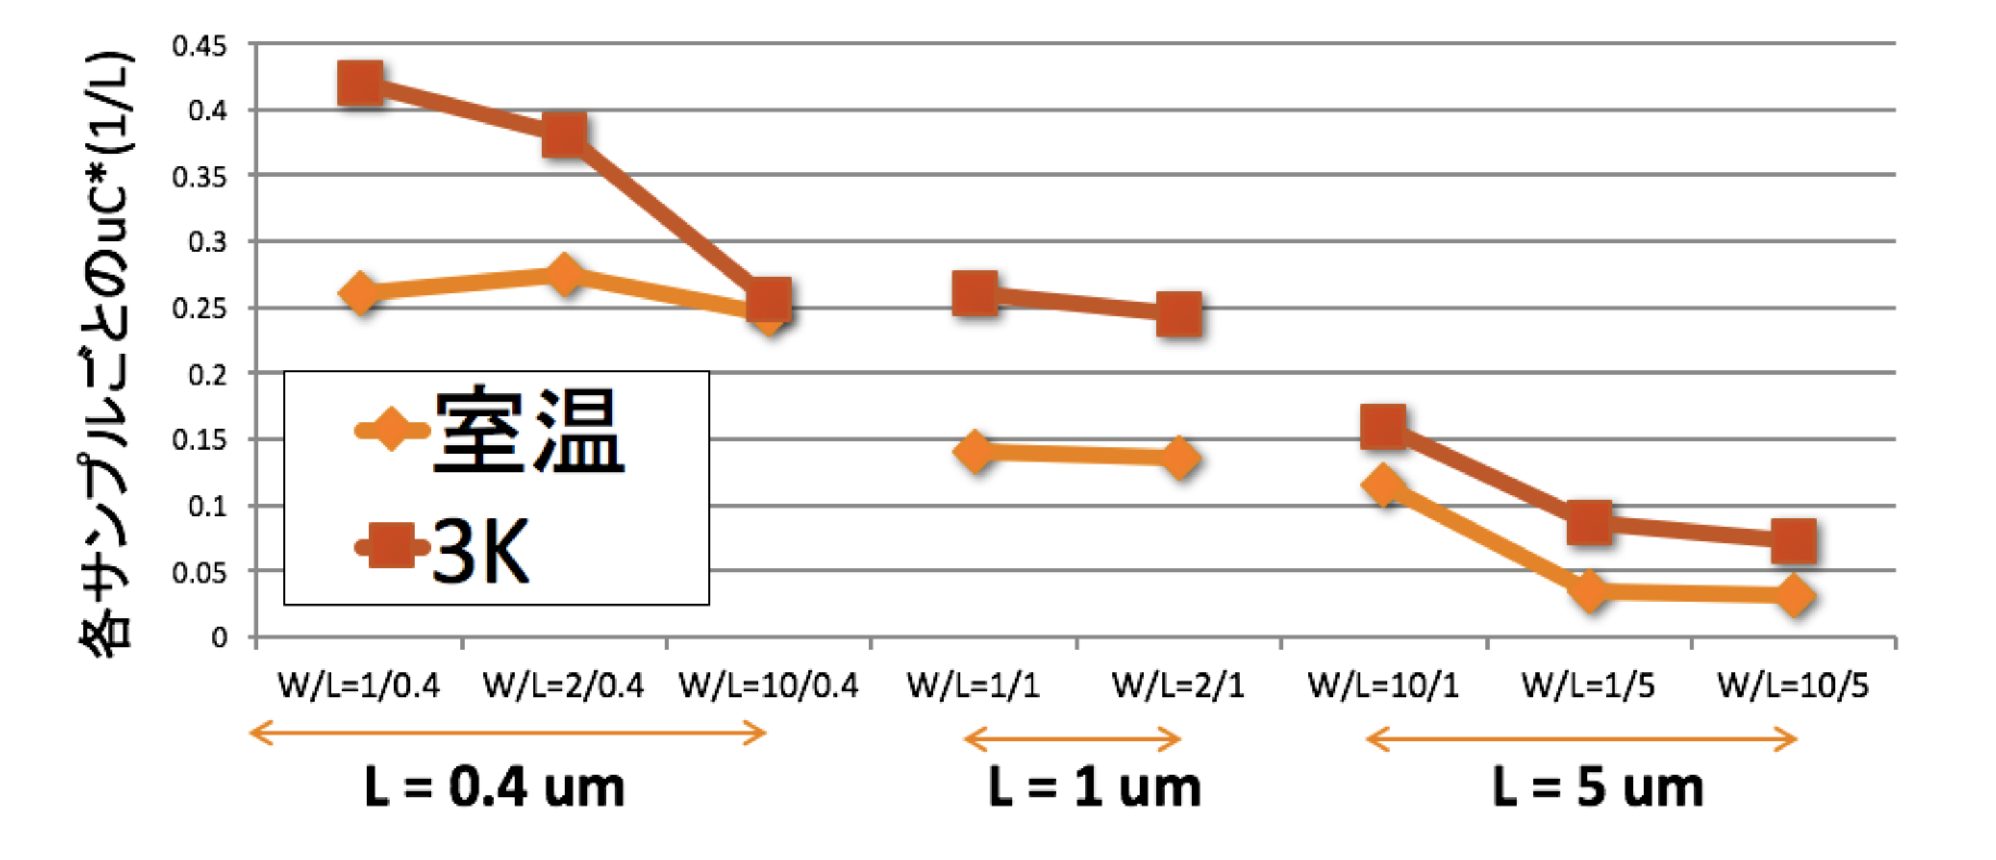
\includegraphics[clip,width=15.0cm]{./Chapter/Appendix/Picture/NST/mu_analysis/mu_analysis_size.eps}
					\caption{各サイズごとの$\mu C_{OX} \frac{1}{L}$値(縦軸:$\mu C_{OX} \frac{1}{L}$ 横:MOSFETのサイズ)}
					\label{fig:mu_analysis_size}
				\end{center}
			\end{figure}
			\clearpage
			
	\section{シミュレーション構築}
		\subsection{シミュレーション}
			我々研究グループが測定したFD-SOI-MOSFETの電流電圧特性の測定結果をもとにJAXA\ 馬場氏にモデリングに必要なパラメータ抽出をしていただいた。
			抽出していただいたパラメータを筑波大PC環境のもとhspice回路シミュレーター、及びngspice回路シミュレーターにて適応させ、シミュレーションを行った。
			
			極低温環境下において、ドレイン電圧$V_{ds}$が低い領域においてドレイン抵抗が異常に大きくなる現象が確認されている。
			この極低温環境特有の特性を現在のMOSFETの電流電圧特性モデルで表現することは不可なので、パラメータ抽出のためのフィッティング領域は飽和領域のみに限定する。
			
			パラメータ抽出を行うトランジスタを表\ref{tab:extract_transistor}にまとめた。
			
			抽出したパラメータをもとにhspiceとngspiceを用いてMOSFETの電流電圧特性のシミュレーションを行い、実測と比較した。
			次節では、その結果について述べる。
			\begin{table}[htb]
				\begin{center}
					\begin{tabular}{| c | c | c |} \hline
						Device Type & Channel Length L & Channel Width \\ \hline \hline
						Body Tie(Nch/Pch) & 0.2$\mathrm{\mu m}$ & 5.0$\mathrm{\mu m}$ \\ \hline
						Source Tie2(Nch/Pch) & 0.4$\mathrm{\mu m}$ & 10$\mathrm{\mu m}$ \\
						\ & 1.0$\mathrm{\mu m}$ & 10$\mathrm{\mu m}$ \\
						\ & 5.0$\mathrm{\mu m}$ & 10$\mathrm{\mu m}$ \\ \hline
					\end{tabular}
					\caption{パラメータ抽出をするトランジスタの一覧}
					\label{tab:extract_transistor}
				\end{center}
			\end{table}
			
		\subsection{シミュレーションと実測の比較}
			\begin{figure}[htbp]
				\begin{center}
					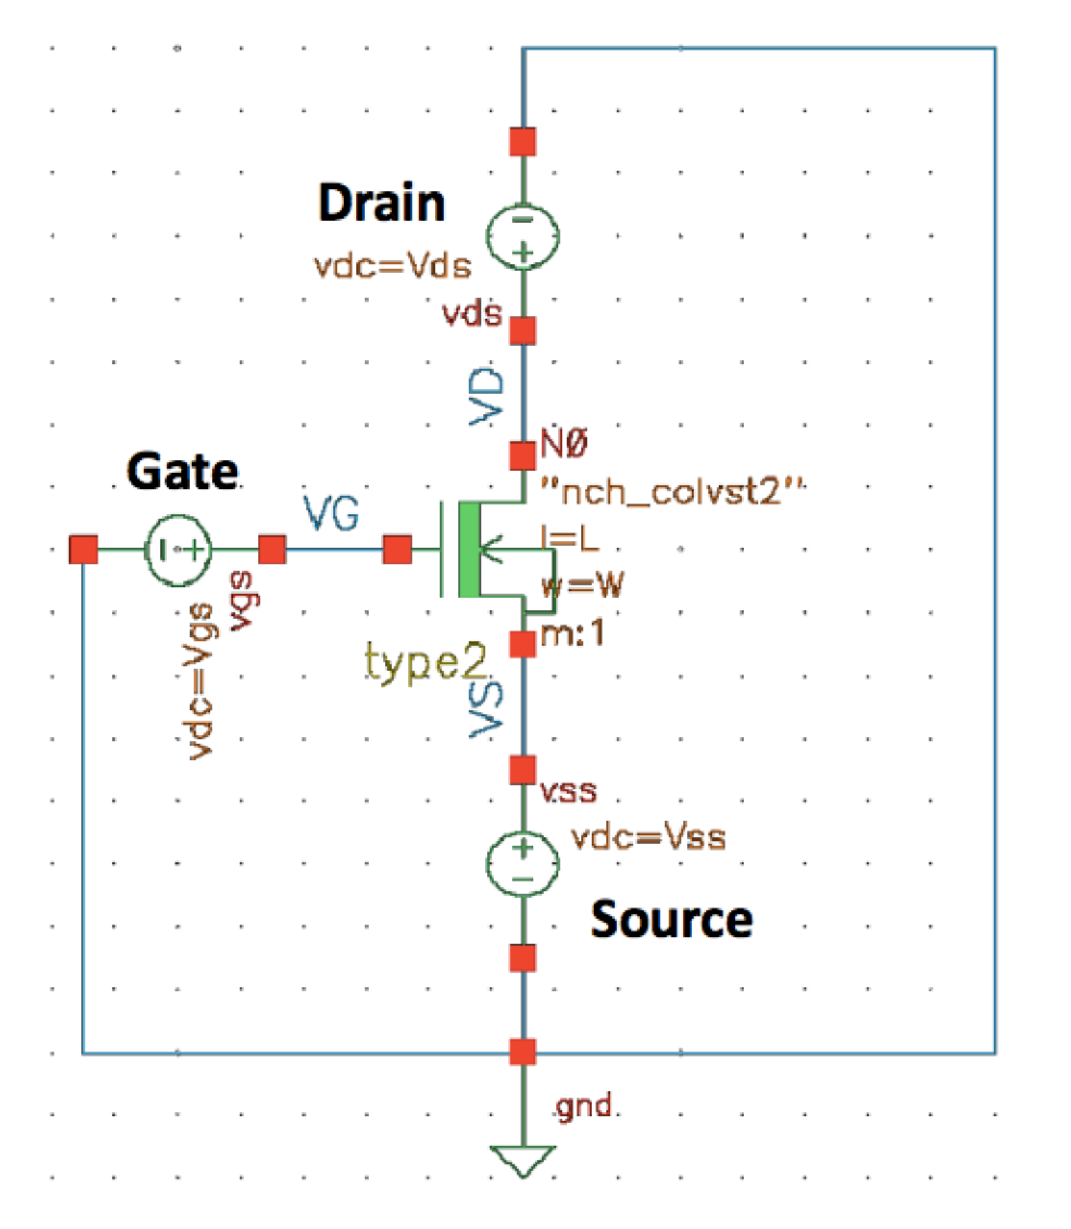
\includegraphics[clip,width=15.0cm]{./Chapter/Chapter5/Picture/simulation_circuit.eps}
					\caption{MOSFETの電流電圧特性シミュレーション回路図}
					\label{fig:simulation_circuit}
				\end{center}
			\end{figure}
			電流電圧特性のシミュレーションの際の回路図を図\ref{fig:simulation_circuit}に示す。そして電流電圧特性についてシミュレーションを行った。
			$I_{ds}-V_{ds}$特性について、極低温環境下での実測とシミュレーションの比較を図\ref{fig:simVSmea_N}と図\ref{fig:simVSmea_P}に示す。
			
			比較すると、NchでもPchでもシミュレーション結果と実測では、
			\begin{itemize}
				\item ドレイン電圧$V_{ds}$が低い領域でのドレイン抵抗異常
				\item 極低温環境下でのキャリア移動度上昇によるKink効果
			\end{itemize}
			について表現できていない。しかし、それを避けた領域での飽和電流値は概ね表現できていることは確認出来る。
			
			以後の設計において、上記のことを踏まえシミュレーションを扱う時には注意を払う必要がある。
			しかし、より精密な設計をするためには、やはり上記の極低温環境下特有の異常特性を抑制し、そしてより精密なシミュレーション構築を行う必要がある。
			
			これら2つの異常特性のうちドレイン抵抗異常特性の抑制について、ドレインとソース間にある低濃度の不純物領域が形成されたLDD(Lightly Doped Drain)構造の不純物濃度を変更することによって、この異常特性を解消することができた。
			次節では、その結果を報告する。
			
			%=====Nch=====%
			\begin{figure}[htbp]
				\begin{center}
					\includegraphics[clip,width=15.0cm]{./Chapter/Chapter5/Picture/simVSmea_N.eps}
					\caption{極低温環境下でのシミュレーションと実測の比較 \newline (Nch-ST2\ W/L=$10\mathrm{\mu m}/0.4 \mathrm{\mu m}$ \ ゲート電圧$V_{gs}=2.0\mathrm{V}$)}
					\label{fig:simVSmea_N}
				\end{center}
			\end{figure}
			%=====Pch=====%
			\begin{figure}[htbp]
				\begin{center}
					\includegraphics[clip,width=15.0cm]{./Chapter/Chapter5/Picture/simVSmea_P.eps}
					\caption{極低温環境下でのシミュレーションと実測の比較 \newline (Pch-ST2\ W/L=$10\mathrm{\mu m}/0.4 \mathrm{\mu m}$ \ ゲート電圧$V_{gs}=-2.0\mathrm{V}$)}
					\label{fig:simVSmea_P}
				\end{center}
			\end{figure}
			\clearpage
			
	\section{LDD不純物濃度改良によるドレイン抵抗異常特性の改善}
		\begin{figure}[htbp]
			\begin{center}
				\includegraphics[clip,width=7.5cm]{./Chapter/Chapter5/Picture/LDD_structure.eps}
				\caption{LDD構造を持つMOSFETの概念図}
				\label{fig:LDD_structure}
			\end{center}
		\end{figure}
		ドレインとソース間にある低濃度の不純物領域のことをLDD(Lightly Doped Drain)構造と呼ぶ。
		この構造は、トランジスタの微細化に伴い、PN接合近傍での電界勾配を緩和するために、ドレイン拡散層の不純物密度分布の勾配も緩やかにするプロセスされている。
		図\ref{fig:LDD_structure}にLDD構造を持つMOSFETの概念図を示した。		
		LDD不純物濃度を濃くしたFD-SOI-MOSFETは、極低温環境下においてのドレイン抵抗異常を抑制することが出来ることが測定で確認できた。
		
		図\ref{fig:LDD_IdVd_P}にLDD不純物濃度を濃くしたPch-ST2型のFD-SOI-MOSFETの$I_{ds}-V_{ds}$特性についての測定結果を示す。
		\begin{figure}[htbp]
			\begin{center}
				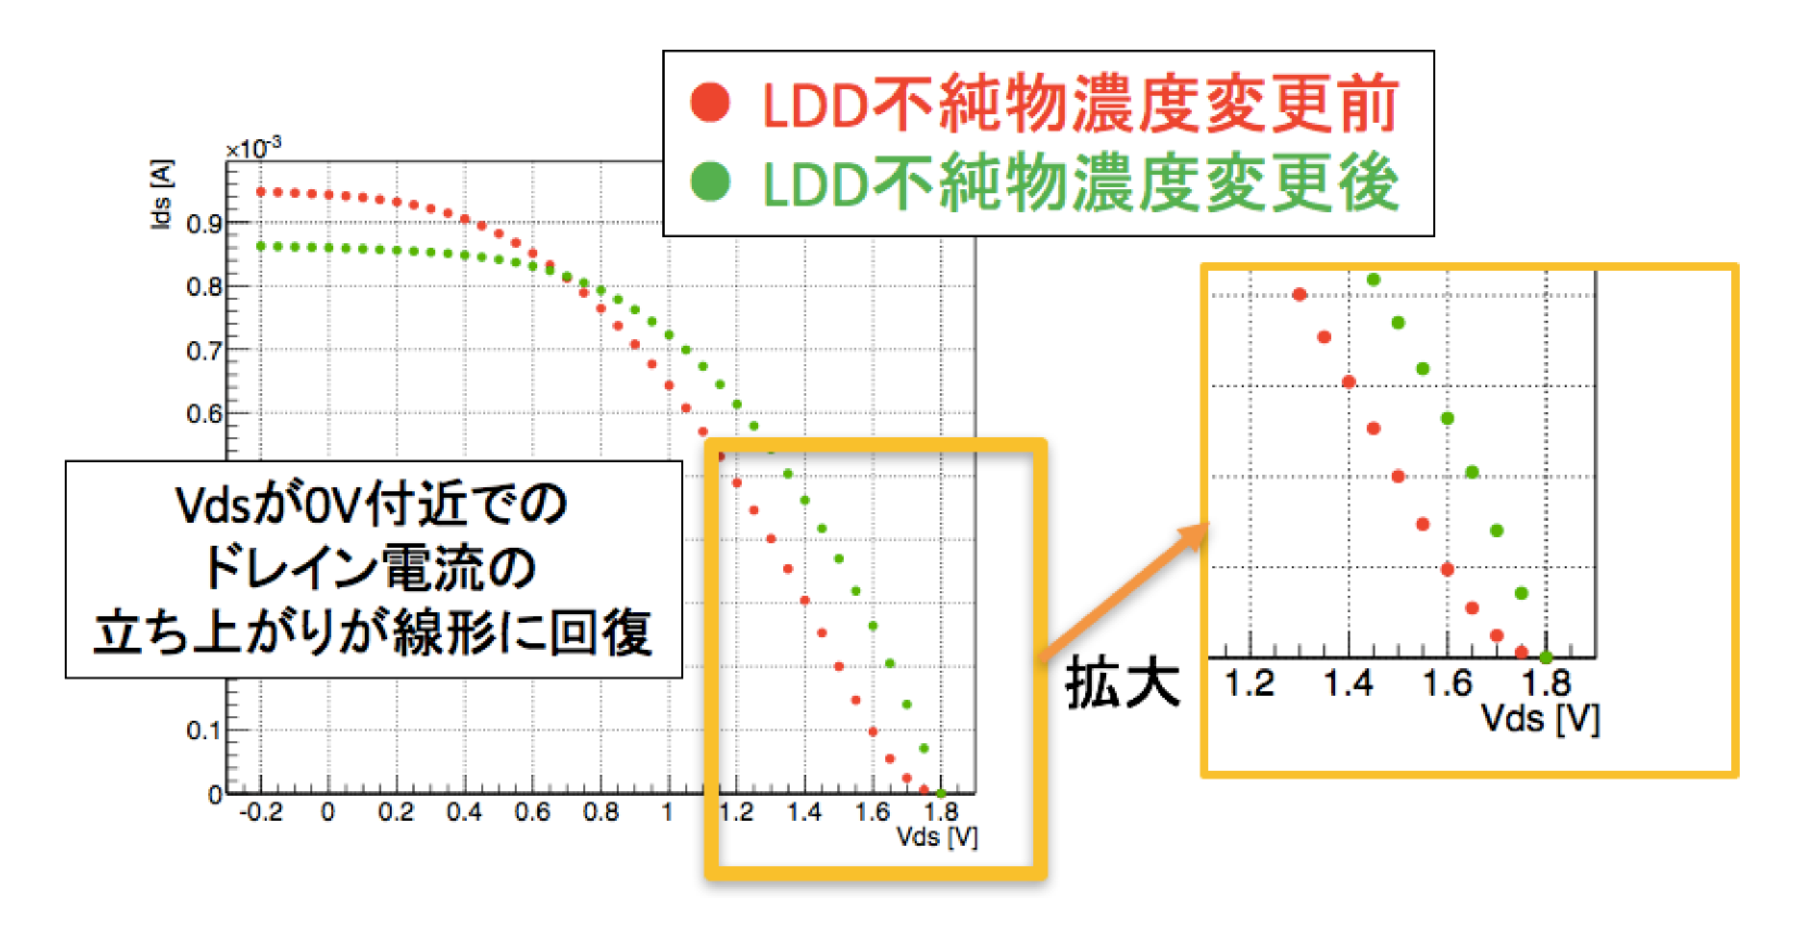
\includegraphics[clip,width=15.0cm]{./Chapter/Chapter5/Picture/LDD_Pch_IdVd_m2.0_W10L1.eps}
				\caption{LDD不純物濃度を改良したPMOSFETの$I_{ds}-V_{ds}$特性(ゲート電圧$V_{gs}=-2.0V$)
					\newline 赤点:不純物濃度改良前\ 緑点:不純物濃度改良後(Pch-ST2型\ $W/L=10\mathrm{\mu m}/1\mathrm{\mu m}$)}
				\label{fig:LDD_IdVd_P}
			\end{center}
		\end{figure}
		
		ドレイン電圧が低い領域を拡大すると、LDD不純物濃度を改良することによってドレイン電流の立ち上がりが線形に回復することがわかる。
		しかし、LDD不純物濃度の変更に伴い、実効的なチャネル長が変動するのでドレイン電流も変動する。
		次回以降のSOI-STJのプロセスにLDD不純物濃度を改良したFD-SOI-MOSFETをプロセスする場合には、LDD不純物濃度変更後の電流電圧特性を知る必要がある。
		
